% Time-stamp: Fri Jul  5 17:05:34 2013
% !TEX root =  free234.tex

\chapter{Parametric curves and vector functions} 

\section{Vector functions} 
So far in calculus we have only considered functions $y=f(x)$ where both the
independent variable $x$ and the dependent variable $y$ are real numbers.

A \emph{vector function} is a function of one variable whose values are vectors
instead of numbers.  One way to specify a vector function is to say what its
components are:
\[
  \vx(t) = \vek x(t) \\ y(t) \\ z(t)\tor = x(t)\ves1 +y(t)\ves2 + z(t)\ves3.
\] 

\section{Using vector functions to describe motion} 
One way to visualize a vector function $\vx(t)$ is to think of the vector
$\vx(t)$ for any given value of $t$ as the position vector of some
point in space (or the plane, if $\vx(t)$ is a two-dimensional vector).  In
other words,  we represent the vector $\vx(t)$ as an arrow starting at the
origin, and ending at some point $X(t)$ whose coordinates are $(x(t), y(t),
z(t))$:
\[
  \vx(t) = \tpv O{X(t)}.
\]
As $t$ varies, the point $X(t)$ moves around and traces out a curve.  Such a
curve is called a \emph{parametrized curve,} or a \emph{parametric curve}.  The
quantity $t$ is called the \emph{parameter.}

We will now take a look at some examples of parametric curves.
\begin{figure}[h]
  \input ../figures/234/01parametric-curve.pdf_tex
  \caption{\textbf{A parametric curve:}  as the parameter $t$ changes, the vector
  $\vx(t)$ will also move.  Keeping the initial point of the vector $\vx(t)$ at
  the origin $O$, the endpoint $X(t)$ traces out a space curve.}
  \label{fig:parametric-curve}
\end{figure}

\section{Lines} 
\label{sec:straight-line-constant-velocity}%
Consider the parametric curve given by
\begin{equation}
  \vx(t) = \va + t\vv
  \label{eq:straight-line-constant-velocity}
\end{equation}
where $\va$ and $\vv$ are given constant vectors.  As before we let
$X(t)$ be the point with $\vx(t) = \tpv O{X(t)}$, i.e.~$\vx(t)$ is the
position vector of the point $X(t)$, and as $t$ changes, $X(t)$ traces
out the parametric curve.

To see what the parametric curve looks like, we let $A$ be the point
with $\tpv OA = \va$, then, since
\[
\tpv O{X(t)} = \tpv OA + \tpv A{X(t)},
\]
it follows from \eqref{eq:straight-line-constant-velocity} that $\tpv
A{X(t)} = t\vv$.  Now consider going from the origin $O$ to the point
$X(t)$ in two steps: first move from $O$ to the point $A$, then go
from $A$ to $X(t)$.  The displacement in the second step is $\tpv
A{X(t)} = t\vv$.  Changing $t$ will then make the point $X(t)$ slide
along the line through the point $A$ in the direction of $\vv$.
\begin{figure}[h]
  \centering \input ../figures/234/01linear-motion2.pdf_tex
  \caption{Vector form of linear motion given by $\vx(t) = \va+t\vv$.}
  \label{fig:vector-form-linear-motion}
\end{figure}

We say that $\vx(t)$ given by
\eqref{eq:straight-line-constant-velocity} describes motion with
constant velocity, whose velocity vector is $\vv$.


\section{Circular motion} 
For given constants $R>0$ and $\omega$ we consider the vector function
\begin{equation}
  \vx(t) = R\cos\omega t \ves1 + R\sin\omega t \ves2
  = \vek R\cos\omega t \\ R\sin \omega t\tor.
  \label{eq:constant-angluar-velocity-on-circle}
\end{equation}
\begin{figure}[h]
  \input ../figures/222/06circle.pdf_tex
  \caption{Circular motion with angular velocity $\omega$.}
  \label{fig:circular-motion}
\end{figure}
The corresponding point is $X(t) = \bigl(R\cos \omega t,  R\sin \omega t\bigr)$.
It lies on the circle of radius $R$ with center at the origin, and the angle
subtended by $OX(t)$ and the positive $x$-axis is exactly $\omega t$.

If $\omega>0$ then as $t$ increases, the angle $\omega t$ increases and the
point $X(t)$ goes around the circle in counter-clockwise direction.  If
$\omega<0$ then $X(t)$ goes around in the clockwise direction.

The number $\omega$ is the rate of increase of the angle $\omega t$, and is
called the \emph{angular velocity} of the motion.

\section{The cycloid} 
% We don't even mention this:
%%%The cycloid is the brachistochrone
%%%The cycloid is the tautochrone
%%%The cycloid is its own evolute
%Perhaps in lecture? 
The \emph{cycloid} is the curve we get if we put a (bicycle) wheel on the
ground, mark the point on the tire that touches the ground, and follow this point
as we roll the wheel forward.  If we call the point $X$, then it depends on the
angle $\theta$ that the wheel has turned since $X$ was on the ground.
Figure~\ref{fig:cycloid} provides a derivation of the vector function
$\vx(\theta) = \tpv O{X(\theta)}$ that describes the cycloid.  The result is
\begin{equation}
  \vx(\theta) = \vek R\theta - R\sin\theta \\ R-R\cos\theta\tor.
  \label{eq:cycloid}
\end{equation}
\begin{figure}[h]
  \input ../figures/234/06cycloid.pdf_tex
  \caption{\textbf{The cycloid. }  A wheel of radius $R$ rolls over the $x$-axis.
  Initially the wheel touches the $x$-axis at the origin $O$.  The cycloid is the
  curve traced out by a point $X$ on the wheel.\\
  \null\qquad\textbf{Derivation of the cycloid motion. }  The arc $AX$ and
  the line segment $OA$ have the same length.  Since $AX$ has length
  $R\theta$, the $x$ coordinates of the points $A$, $B$, and $C$ are $R\theta$.
  The right triangle $CXB$ has hypotenuse $R$, so the lengths of $XB$ and $CB$
  are $R\sin\theta$, and $R\cos\theta$, respectively.  Therefore the coordinates
  of the point $X$ are $x=R\theta - R\sin\theta$, and $y=R-R\cos \theta$.}
  \label{fig:cycloid}
\end{figure}

\section{The helix}  
\label{sec:helix}
When we walk up a spiral staircase we are tracing out a helix:  we are going
around in circles, and moving upward at the same time.  The parametric curve
that does this (and that has the $z$-axis as its central axis) is given by
\begin{equation}
  \vx(\theta) = \vek R\cos \theta \\ R\sin \theta\\ a \theta\tor
  \quad
  \text{or: }\quad
  \vx(\theta) = R\cos\theta\ves1+R\sin\theta\ves2 +a\theta\ves3.
  \label{eq:helix-def}
\end{equation}
Here $R>0$ is the radius of the helix, i.e.~the radius of the circle on the
ground above which the helix lies;  the number $a$ represents the rate at which
the helix goes up.
\begin{figure}[h]
  \centering
  \input ../figures/234/01helix.pdf_tex
  \caption{\textbf{The Helix. } The point $X$ traces out a helix: it sits at a
  height $a\theta$ above the point $Y$, while $Y$ runs around on a circle of radius
  $R$; here $\theta = \angle AOY$}
  \label{fig:helix}
\end{figure}

\section{The derivative of a vector function} 

For a function $y=f(x)$ of one variable we had two ways of describing the
derivative:  on one hand we had a geometric description of $f'(x)$ as ``the
slope of the tangent to the graph,'' and on the other we could describe $f'(x)$
in terms of a difference quotient, i.e.
\[
  f'(x) = \lim_{\Delta x\to0} \frac{f(x+\Delta x) - f(x)}{\Delta x}.
\]
For vector functions we can imitate both descriptions.  We begin with the formal
definition in terms of limits and then proceed to the geometric description, in
which we interpret the derivative as the ``instantaneous velocity vector.''


\subsection*{Definition}
If $\vx(t)$ is a vector function, then we set
\begin{equation}
  \vx'(t) \stackrel{\rm def}= \lim_{\Delta t\to0} \frac{\vx(t+\Delta t)
    - \vx(t)}{\Delta t}.
  \label{eq:vector-derivative-def}
\end{equation}
For \eqref{eq:vector-derivative-def} to make sense we would have to define what
the limit of a vector function is.  This can be done, but we will not go into the
precise definitions in this course.  More important for our use is that if the
components of a vector function $\vx(t)$ are given, then the derivative can be
computed by just differentiating those components:
\begin{equation}
  \vx'(t) = \vek
  x'(t) \\ y'(t) \\z'(t)
  \tor,
  \quad\text{or}\quad
  \vx'(t) = x'(t)\ves1 +y'(t)\ves2 +z'(t)\ves3.
  \label{eq:derivative-of-vector-function}
\end{equation}
As with ordinary functions of one variable we will use Leibniz' notation for the
derivative whenever it seems convenient.  Thus the following are equivalent ways
of expressing the same derivative:
\[
  \va'(t) = \frac{d\va(t)}{dt} = \frac{d}{dt}\va(t).
\]
\subsection*{Example} For instance, 
\[
  \vx(\theta) = \vek\cos \theta \\ 0 \\\theta\tor
  = \cos\theta\,\ves1 + \theta\,\ves3
\]
defines a vector function.  Here we have called the independent variable $\theta$
instead of $t$.  The derivative of this vector function is
\[
  \frac{d\vx}{d\theta}
  = \frac{d}{d\theta} \vek\cos \theta \\ 0 \\\theta\tor
  = \vek - \sin\theta \\ 0 \\ 1 \tor
  = -\sin\theta\,\ves1 + \ves3.
\]

\begin{figure}[b]
  \centering
  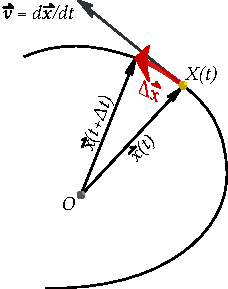
\includegraphics{01velocityistangent.pdf}
  \caption{%
  The vector function $\vx(t)$ traces out a curve in space.  The vector
  $\vx(t)$ is the position vector of a point $X(t)$ on this curve.  As we
  increase time from $t$ to $ t+\Delta t$, the point $X(t)$ moves.  The
  displacement of the point $X(t)$ is given by $\Delta\vx = \vx(t+\Delta t) -
  \vx(t)$.  The average velocity vector during this displacement is
  ``displacement/time'', i.e.\ $\Delta \vx/\Delta t$.\\
  %
  \null\qquad If we let $\Delta t\to 0$, then the average velocity becomes the
  instantaneous velocity at time $t$: $\vv = \lim_{\Delta t\to0}\Delta\vx/\Delta
  t = \vx'(t)$.  This vector is tangent to the curve traced out by the vector
  function $\vx(t)$. We call it a \emph{tangent vector}.
  }
  \label{fig:05velocity-is-deriv-of-position}
\end{figure}
\section{The derivative as velocity vector} 
\label{sec:velocity-of-vector-motion}
Suppose the motion of some point $X(t)$ in space is described by its position
vector function $\vx(t)$.  Let us try to define the instantaneous velocity of
the point.  This velocity should have magnitude (``how fast the point is
moving'') and also direction (``which way is the point going?'').  The velocity
should therefore be a vector.  To see which vector, we go back to the notion
that ``velocity'' is always ``displacement divided by time.''

We consider two instances in time, say, time $t$ and time
$t+ \Delta t$.  Then the position vectors of the point $X$ at these
two different times are $\vx(t)$ and $\vx(t+\Delta t)$.  The
displacement of the point $X$ between these two times is then
\[
\Delta \vx = \vx(t+\Delta t) - \vx(t)
\]
(see Figure~\ref{fig:05velocity-is-deriv-of-position}.)  We say that
the average velocity over the time interval from $t$ to $t+\Delta t$
is ``the displacement divided by $\Delta t$,'' i.e.
\[
\vv_{\rm average} = \frac{\vx(t+\Delta t) - \vx(t)}{\Delta t}.
\]
Note that the average velocity is a vector.  If we write it out in
components, we get a much larger formula:
\[
\vv_{\rm average} = \vek
\dfrac{x(t+\Delta t) - x(t)}{\Delta t} \\[2ex]
\dfrac{y(t+\Delta t) - y(t)}{\Delta t} \\[2ex]
\dfrac{z(t+\Delta t) - z(t)}{\Delta t} \tor.
\]
One big advantage of using vector notation is that many formulas simplify
considerably when written in terms of vectors.

To get the instantaneous velocity, we do the same thing as in one
variable calculus: we take the limit as $\Delta t\to0$ of the average
velocity over the time interval from $t$ to $t+\Delta t$.  Thus we get
\begin{equation}
  \vv(t) = \lim_{\Delta t\to0} \frac{\vx(t+\Delta t) - \vx(t)}{\Delta t}
  \stackrel{\rm def}=
  \frac{d\vx}{dt}.
  \label{eq:velocity-of-vector-motion}
\end{equation}
In terms of components this derivative is
\[
\vx'(t)= \frac{d\vx}{dt} = \vek x'(t) \\ y'(t) \\ z'(t) \tor.
\]
Thus the velocity vector of any given vector function $\vx(t)$ is the same as
the derivative of this vector function.

\section{Acceleration} 
Having found the velocity vector of a point $X(t)$ whose position vector is a
given vector function $\tpv O{X(t)} = \vx(t)$, we can also define the
\emph{acceleration vector} of the moving point.  By definition, the acceleration
vector is the derivative of the velocity vector, i.e.
\begin{equation}
	\va(t)
	= \frac{d\vv}{dt}
	= \frac{d^2\vx} {dt^2} = \vek x''(t)\\ y''(t) \\ z''(t) \tor.
	\label{eq:acceleration-vector-def}
\end{equation}
This definition is entirely analogous to the definition of acceleration
(``$a=\frac{dv}{dt}$'') from first semester calculus.  The only difference is
that, here, the position, velocity, and acceleration all have directions in
addition to magnitudes:  they are vectors.

Newton's famous law relating forces and acceleration continues to hold.  If a
point $X(t)$ moves according to some vector function $\vx(t)$, then some force
must be acting on this point. This force is a vector (it has magnitude and
direction), and, according to Newton, it is given by
\begin{equation}
  \vF = m\va = m\frac{d\vv}{dt} = m \frac{d^2 \vx}{dt^2},
  \label{eq:SirIsaacs-law}
\end{equation}
where $m$ is the mass of the object at the point $X(t)$ whose motion we are
considering.  It is always assumed to be a positive number.

Note that according to this law, the absence of forces, i.e.~$\vF=\vvv0$, is the
same as $\frac{d\vv}{dt}=\vvv0$, i.e.~no force acts on the point if and only if
its velocity vector is constant.  Here ``constant'' means constant magnitude
\emph{and} constant direction.

\section{The differentiation rules} 
Just as with ordinary derivatives, the derivatives of vector functions satisfy
certain rules, such as the product rule.  The purpose of these rules is not the
same as in one variable calculus.  There we used sum, product, quotient and
chain rules to compute derivatives of given functions without having to fall
back on the definition of a derivative all the time.  For vector functions we
do not need such rules, because we can differentiate them by simply differentiating
each of their components (see the above example).   Instead, the differentiation
rules for vector functions are mostly used to gain insight and establish general
facts about vector functions, a number of which we will see shortly.  

\subsection{The sum rule} 
The analog of the sum rule (``derivative of the sum is the sum of the
derivatives'') looks exactly like the ordinary sum rule.  It says that for any
two vector functions $\va(t)$ and $\vb(t)$ one has
\[
  \frac{d}{dt}\bigl(\va(t) \pm \vb(t)\bigr) 
  =\frac{d\va(t)}{dt} \pm \frac{d\vb(t)}{dt}.
\]

\subsection{The many product rules} 
There is no quotient rule for vector functions, simply because we have no way of
dividing vectors.  On the other hand we have two ways of multiplying vectors,
and we can also multiply vectors and numbers, so there are \emph{three}
different product rules.  Fortunately they all look like the product rule from
first semester calculus.

If $\va(t)$ and $\vb(t)$ are vector functions, and if $f(t)$ is a function,
then
\begin{align*}
  \frac{d \va(t)\dpp \vb(t)}{dt}
  &= \frac{d\va(t)}{dt} \dpp\vb(t) + \va(t) \dpp \frac{d\vb(t)}{dt}\\[1ex]
  \frac{d \va(t)\cp \vb(t)}{dt}
  &= \frac{d\va(t)}{dt} \cp\vb(t) + \va(t) \cp \frac{d\vb(t)}{dt}\\[1ex]
  \frac{d\,f(t) \va(t)}{dt}
  &= \frac{df(t)}{dt} \va(t) + f(t)  \frac{d\va(t)}{dt}
\end{align*}
In spite of the fact that these rules ``look right,'' they could still be wrong,
so to be sure we would have to prove them.  The proofs are very straightforward.
Here is a short proof for the product rule involving the dot product.  To
shorten the formulas we omit the ``$(t)$'' from all functions:
\begin{align*}
  \frac{d\va\dpp\vb}{dt}
  &= \frac{d}{dt}\bigl(a_1b_1+a_2b_2\bigr) \\
  &= \frac{da_1b_1}{dt} + \frac{d a_2b_2}{dt} \\
  &= \frac{da_1}{dt}b_1 + {\color{blue}a_1 \frac{db_1}{dt} }
  +{\color{red}\frac{da_2}{dt}b_2} + a_2 \frac{db_2}{dt}
  &\text{\footnotesize\sffamily ordinary product rule}\\
  &= \frac{da_1}{dt}b_1 + {\color{red}\frac{da_2}{dt}b_2}
    + {\color{blue}a_1 \frac{db_1}{dt} } + a_2 \frac{db_2}{dt} 
  &\text{\footnotesize\sffamily switch terms around}\\
  &= \frac{d\va}{dt}\dpp\vb + \va\dpp \frac{d\vb}{dt}.
  &\text{\footnotesize\sffamily recognize the dot-products}\\
\end{align*}


\section{Vector functions of constant length} 
\label{sec:vector-functions-of-constant-length}
As an immediate application of the product rule for the dot-product we prove the
following fact about vector functions whose length does not change, i.e.~vector
functions $\va(t)$ that change their direction, but not their length.

\null\hfill
\begin{minipage}[b]{0.4\textwidth}
\input ../figures/234/01constant-length-vector-function.pdf_tex
\end{minipage}\hfill
\begin{minipage}[b]{0.4\textwidth}\sffamily\color{darkbluegreen}
  \rule{\textwidth}{1pt}

  If a vector function $\va(t)$ has constant length, then, when the parameter $t$
  undergoes a small change $\Delta t$, the corresponding small change $\Delta \va$
  in the vector function will be almost perpendicular to $\va(t)$ itself.

  \rule[1ex]{\textwidth}{1pt}
\end{minipage}
\hfill\,
\medskip


\subsubsection*{Theorem}\itshape Let $\va(t)$ be a vector function.  Then a
necessary and sufficient condition for the length $\|\va(t)\|$ to be constant is
that $\va(t)$ and $\va'(t)$ be perpendicular for all $t$.\upshape

\begin{proof}
Differentiating both sides of the equation
\[
  \|\va(t)\|^2 = \va(t) \dpp \va(t)
\]
we get
\begin{equation}
  \frac{d}{dt}\|\va(t)\|^2 =
  \va'(t) \dpp \va(t) + \va(t) \dpp \va'(t)
  =2\va(t) \dpp \va'(t).
  \label{eq:derivative-of-squared-length}
\end{equation}
If $\va(t)$ has constant length, then $\|\va(t)\|^2$ is also constant, and thus
$\tfrac d{dt} \|\va(t)\|^2 = 0$.   Therefore, for a vector function $\va(t)$
whose length is constant, $\va(t)\dpp\va'(t)=0$, i.e.~$\va(t)\perp\va'(t)$.

Conversely, if $\va(t)$ is a vector function for which $\va(t)\perp\va'(t)$
holds for all $t$, then $\va(t)\dpp\va'(t)=0$, and
\eqref{eq:derivative-of-squared-length} implies that $\tfrac d{dt} \|\va(t)\|^2
= 0$, i.e.~that $\|\va(t)\|^2$ and hence $\|\va(t)\|$ are constant.  

\end{proof}

\section{Two examples} 
\subsection{Motion on a straight line} 
We return to the motion given by \eqref{eq:straight-line-constant-velocity},
i.e.
\begin{equation}
  \vx(t) = \va + t\vv.
\end{equation}
The velocity and acceleration are easy to compute:
\[
 \frac{d\vx(t)} {dt} = \vv, \qquad
 \frac{d^2\vx(t)} {dt} = \frac{d\vv} {dt} = \vvv0,
\]
since $\vv$ is a constant vector in this case.  

We see that if a point $X(t)$ moves according to the parametrization
\eqref{eq:straight-line-constant-velocity}, then its velocity is
constant, and its acceleration is zero.  According to Newton's law, no
force is exerted on an object undergoing this motion.

\subsection{Circular motion} 
For the point $X(t)$ moving on a circle of radius $R$ with angular velocity
$\omega$ we have \eqref{eq:constant-angluar-velocity-on-circle}, i.e.
\[
  \vx(t) = R\cos\omega t \ves1 + R\sin\omega t \ves2
\]
so that the velocity and acceleration are easy to compute:
\begin{center}
  \begin{tabular}{r@{}r@{}c@{}r}
    $\vv(t) =\vx'(t) =$\;   %%%%%%%%%%%%%%%%%%%%%%%%%%%% row 1
    &$-\omega R\sin \omega t\;\ves1$
    & $+$\;&$\omega R\cos \omega t\;\ves2$,\\
    $\va(t) =\vv'(t) =$\;   %%%%%%%%%%%%%%%%%%%%%%%%%%%% row 2
    &$-\omega^2R\cos\omega t\;\ves1$
    & $-$\;&$\omega^2R\sin \omega t\;\ves2$. 
  \end{tabular}
\end{center}

Note that the velocity vector $\vv(t)$ is perpendicular to the position
vector $\vx(t)$, as predicted in
\S~\ref{sec:vector-functions-of-constant-length}.
Our expression for the velocity vector $\vv(t)$ contains the familiar relation
between angular velocity and velocity:  the velocity $v=\|\vv(t)\|$ with which
the point $X(t)$ is moving is 
\begin{align}
  \label{eq:speed-of-circular-motion}
  v(t) &= \left\|-\omega R\sin \omega t\;\ves1
    +\;\omega R\cos \omega t\;\ves2\right\|  \\
    &= \sqrt{\omega^2R^2\sin^2\omega t + \omega^2R^2\cos^2\omega t}\notag \\
    &= \omega R.\notag
\end{align}
Hence the angular velocity of an object undergoing circular motion is
\begin{equation}
  \omega = \frac{v}{R}.
  \label{eq:angular-from-regular-velocity}
\end{equation}
\begin{figure}[h]
  \input ../figures/222/06circle3.pdf_tex
  \caption{If an object moves along a circle with constant angular velocity,
  then the acceleration $\vF$ required to make the object follow that motion is $\va =
  -\omega^2 \vx$.  In particular it is parallel to the position vector $\vx$
  but in the opposite direction. }
  \label{fig:circular-motion-the-force}
\end{figure}


We also note that the acceleration is a multiple of the position vector:
\[
  \va(t) = -\omega^2 \vx(t).
\]
According to Newton the force acting on the object at $X(t)$ is $\vF = m\va =
-m\omega^2\vx$, and its magnitude is
\begin{equation}
  F = \|\vF\| = \|m\omega^2\vx(t)\| = m\omega^2R,
  \label{eq:centrifugal-force}
\end{equation}
because $\|\vx(t)\|=R$ at all times.

Using \eqref{eq:angular-from-regular-velocity} we can replace the angular velocity
$\omega$ by the actual velocity, which leads to the classical formula for the
centrifugal force
\begin{equation}
  F = \frac{mv^2}{R}.
  \label{eq:centrifugal-force-from-velocity}
\end{equation}

\section{Arc length} 
\label{sec:arc-length}
For any given vector function there is a simple formula for the length of the curve
it traces out.  The formula is essentially the same as the formula for the length of
a parametric curve (or, to a lesser extent, of the graph of a function) that was
described in Math 221.  Here we repeat the intuitive derivation of the formula,
written in terms of vectors this time.

Let $\vx(t)$ ($a\le t\le b$) be a vector function.  To determine the length of the
arc traced out by $X(t)$ as $t$ varies from $t=a$ to $b$, we divide the interval
$a\le t\le b$ into many very short subintervals.  The corresponding points $X(t)$ on
the curve split the curve into many short segments, each of which will be ``close to
a line segment.''  We approximate the length of the curve by adding the lengths of
all these short segments.  Finally we take the limit in which the number of partition
points becomes infinite and our sum of lengths of short segments becomes an integral.
To see which integral we get, we need to find an expression for the length of a short
segment between two adjacent partition points on the curve.

Suppose we have two points on the curve, with parameter values $t$ and $t+\Delta t$,
respectively.  The points are $X(t)$ and $X(t+\Delta t)$, and the distance between
them is the length of the vector $\Delta\vx$ from one point to the next.
\marginpar{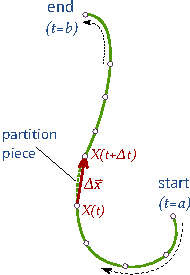
\includegraphics{01length-of-curve.pdf}}%
This vector is
\[
\Delta x = \vx(t+\Delta t) - \vx(t) =\frac{ \vx(t+\Delta t) - \vx(t)}{\Delta t} \;
\Delta t \approx \vx'(t) \Delta t,
\]
so that its length is $\approx \|\vx'(t)\| \, \Delta t$.  Adding the lengths of the
short segments together, we find that the length is approximately $\sum \|\vx'(t)\|
\, \Delta t$ (where the summation is over all short pieces of the curve).  Taking the
limit we arrive at this formula for the length of the curve traced out by $\vx(t),
a\le t\le b$:
\begin{equation}
  \text{Length} = \int_{t=a}^b \|\vx'(t)\|\; dt.
  \label{eq:length-of-curve-vector-version}
\end{equation}

This integral looks simple, but that appearance turns out to be deceptive as we find
out when we write it in terms of the components of the vector function $\vx(t)$.
Suppose $\vx(t) = x(t)\ves1 + y(t)\ves2 + z(t)\ves3$.  Then
\[
\vx'(t) = x'(t)\ves1 + y'(t)\ves2 + z'(t)\ves3,
\]
so that
\[
\|\vx'(t)\| = \sqrt{x'(t)^2 + y'(t)^2 +z'(t)^2}.
\]
Therefore the length formula \eqref{eq:length-of-curve-vector-version} of the curve
is equivalent to
\begin{equation}
  \label{eq:length-of-curve-in-components}
  \text{Length} = \int_{t=a}^b \sqrt{x'(t)^2 + y'(t)^2 +z'(t)^2}\; dt.
\end{equation}
The square root makes this formula a reliable source of very difficult integrals.  In
fact the list of curves whose length one can actually compute by doing the integral
is rather short (see Problem ...).

\section{Arc length derivative} 
Let $\vx(t)$ be some vector function that describes the motion through space of some
point $X(t)$, and let $f(t)$ be some other function.  In what follows it will help to
think of the parameter $t$ as ``time.''  Typical examples of functions $f$ that we
might want to consider are $f(t) = \|\vx(t)\|$ (the distance to the origin of the
point $X(t)$) or $f(t) = \|\vx'(t)\|$ (the speed at which the point is moving.)

To describe the rate with which $f(t)$ is changing we could compute its derivative,
\[
  \frac{df}{dt}
\]
which tells us what the ratio between the change $\Delta f$ of $f$, and the change
$\Delta t$ in the parameter $t$ is (at least approximately, if $\Delta t$ is small).
If we interpret $t$ as ``time'' then this derivative tells us how fast $f(t)$ changes
per second.  But sometimes it is more useful to know how much $f$ changes after we
have travelled a small \textit{distance} along the curve, rather than after a short
amount of time has passed.  In other words, for two nearby points $X(t)$ and
$X(t+\Delta t)$ on the curve we would like to know the ratio
\begin{equation}
  \frac{\text{change in $f$}}{\text{distance travelled}}=
  \frac{f(t+\Delta t) - f(t)}{\text{distance from $X(t)$ to $X(t+\Delta t)$}}
  \label{eq:ratio-Df-Ds}
\end{equation}
We can work this out by observing that the distance from $X(t)$ to $X(t+\Delta t)$ is
the length of the vector from  $X(t)$ to $X(t+\Delta t)$, i.e.
\[
{\text{distance from $X(t)$ to $X(t+\Delta t)$}}
=
\left\|\vx(t+\Delta t) - \vx(t)\right\|.
\]
Assuming $\Delta t$ is small, we have
\[
\left\|\vx(t+\Delta t) - \vx(t)\right\|
=
\left\|\frac{\vx(t+\Delta t) - \vx(t)}{\Delta t}\right\|\; \Delta t
\approx
\left\|\vx'(t)\right\|\; \Delta t.
\]
We substitute this in \eqref{eq:ratio-Df-Ds}, and get
\[
  \frac{\text{change in $f$}}{\text{distance travelled}}
  \approx
  \frac{f(t+\Delta t) - f(t)}{\|\vx'(t)\| \Delta t}.
\]
Now let $\Delta t\to0$:  the quantity on the left becomes what is called the
\emph{arc length derivative} of the function $f$ along the curve
$\vx(t)$, and which is commonly denoted by $\frac{df}{ds}$
In the quantity on the right we recognize the derivative of $f$ with respect
to $t$ (time), which leads to
\begin{equation}
  \frac{df}{ds} = \frac{1}{\|\vx'(t)\|}\, \frac{df}{dt}.
  \label{eq:arclength-derivative-vs-time-derivative}
\end{equation}
Here $\frac{df}{dt} = f'(t)$ is the usual derivative of $f$ with respect to $t$.

If we want to emphasize the distinction between these two derivatives, then we can
call $\frac{df}{dt}$ the ``time derivative of $f$.''

\section{Unit Tangent and Curvature} 
\subsection{Unit tangent} 
We have seen that we can find a tangent vector to the curve traced out by some vector
function $\vx(t)$, simply by differentiating the vector function:  $\vx'(t)$ always
provides a tangent vector (if $\vx'(t)\ne \vvv0$).  
\marginpar{\sffamily\footnotesize%
\color{darkbluegreen}A vector with length 1 is called a \emph{unit vector}}%
In fact any multiple $\lambda\vx'(t)$ of this vector will also be a tangent
vector (provided $\lambda\ne0$.)  We can single out one special tangent vector,
by choosing $\lambda>0$ so that $\lambda\vx'(t)$ has length 1.  Since for
$\lambda>0$ we have $\|\lambda \vx'(t)\| = \lambda \|\vx'(t)\|$ the value of
$\lambda$ that will make $\lambda\vx'(t)$ a unit vector is $\lambda =
1/\|\vx'(t)\|$.

For this reason the vector
\begin{equation}
  \vT(t) = \frac{d\vx}{ds} = \frac{\vx'(t)}{\|\vx'(t)\|}
  \label{eq:unit-tangent-def}
\end{equation}
is called the \emph{unit tangent vector} to the curve corresponding to the vector
function $\vx(t)$.

\subsection{Example}  For our constant velocity parametrization 
\eqref{eq:straight-line-constant-velocity} of a straight line from
\S~\ref{sec:straight-line-constant-velocity} we have
\[
  \vx(t) = \va+t\vv,
\]
so that $\vx'(t) = \vv$ and hence
\[
  \vT = \frac{\vv}{\|\vv\|}.
\]
We see that the unit tangent vector is constant.

\subsection{Curvature and normal} 
If the curve described by a vector function $\vx(t)$ is not a straight line,
then the tangent to the curve will turn as one moves along the curve.  The
\emph{curvature vector} $\vvv\kappa$ measures how much the curve is curved.  It
is defined to be the rate of change of the unit tangent, but with respect to arc
length instead of with respect to the given parameter $t$.  Thus
\begin{equation}
  \vvv\kappa \stackrel{\rm def}= \frac{d\vT}{ds}.
  \label{eq:curvature-vector-def}
\end{equation}
According to our definition of ``derivative with respect to arc length'' the
right hand side stands for
\begin{equation}
  \frac{d\vT}{ds} = \frac{1}{\|\vx'(t)\|} \frac{d\vT}{dt}.
  \label{eq:curvature-vector-def2}
\end{equation}
To write this completely in terms of the original vector function $\vx(t)$ we
use \eqref{eq:unit-tangent-def}
\begin{equation}
  \vvv\kappa
  = \frac{1}{\|\vx'(t)\|}
  \frac{d}{dt} \Bigl\{\frac{1}{\|\vx'(t)\|}\frac{d\vx}{dt} \Bigr\}
  \label{eq:curvature-vector-in-hideous-form}
\end{equation}
This formula is not as short as the original definition
\eqref{eq:curvature-vector-def}, but it does show that the curvature vector
comes about by differentiating the vector function $\vx(t)$ twice (and dividing
by $\|\vx'(t)\|$ at the right moments.)
\bigskip

\subsubsection*{Theorem}\itshape%
The curvature vector $\vvv\kappa$ is perpendicular to the tangent,
i.e.~$\vvv\kappa\perp\vT$.\upshape

\begin{proof}
We have to show that $\vvv\kappa\dpp\vT=0$.  From the second form
\eqref{eq:curvature-vector-def2} of the definition of $\vvv\kappa$ we see
\[
  \vvv\kappa\dpp\vT = 
  \Bigl(\frac{1}{\|\vx'(t)\|} \frac{d\vT}{dt}\Bigr) \dpp \vT
  =
  \frac{1}{\|\vx'(t)\|} \;  \frac{d\vT}{dt} \dpp \vT \;.
\]
Remember that $\vT(t)$ is always a unit vector, i.e.~$\vT(t)$ has constant
length: by \S~\ref{sec:vector-functions-of-constant-length} this implies that
$\frac{d\vT}{dt}\perp\vT(t)$ and thus $\frac{d\vT}{dt}\dpp\vT=0$, so we are done.
\end{proof}

There are two concepts that are derived from the curvature vector:  the
\emph{curvature} $\kappa$ is by definition the length of the curvature vector
$\vvv\kappa$,
\begin{equation}
  \kappa = \|\vvv\kappa\| = \left\| \frac{d\vT}{ds}\right\|,
  \label{eq:curvature-def}
\end{equation}
and the \emph{normal vector} to the curve is 
\begin{equation}
  \vN = \frac{\vvv\kappa}{\|\vvv\kappa\|} 
  = \frac{\frac{d\vT}{ds}}{\left\|\frac{d\vT}{ds}\right\|}.
  \label{eq:normal-vector-def}
\end{equation}
The normal vector is undefined when $\vvv\kappa=\vvv0$, because it would require
division by zero.

Since $\vvv\kappa$ is perpendicular to $\vT$, the normal vector $\vN$ is also
perpendicular to $\vT$ (hence its name).
\begin{equation}
  \frac{d\vT}{ds} = \kappa\; \vN
  \label{eq:first-Serret-Frenet}
\end{equation}

%%\begin{equation}
%%  \frac{d\vN}{ds} = -\kappa\vT + \tau\; \vB
%%  \label{eq:second-Serret-Frenet}
%%\end{equation}
%%where
%%\[
%%\vB= \vT\cp\vN.
%%\]
%%\begin{equation}
%%  \frac{d\vB}{ds} = -\tau\; \vN
%%  \label{eq:third-Serret-Frenet}
%%\end{equation}

\section{Osculating plane} 
At any point $X(t)$ on a space curve given by $\vx(t)$ one defines the
\emph{osculating plane} to be the plane that contains the point $X(t)$ and that
is parallel to both the tangent $\vT(t)$ and normal $\vN(t)$ of the curve.

If we want to write a defining equation for the osculating plane as in
\S~\ref{sec:defining-eq-planes} then we need a vector perpendicular to the
osculating plane.  Since this plane is defined to be parallel to both $\vT$ and
$\vN$, we can find a normal vector to the osculating plane by taking the cross
product of $\vT$ and $\vN$.  This vector is called the \emph{binormal} to the
curve.  In a formula, it is defined to be
\begin{equation}
  \vB = \vT\cp\vN .
  \label{eq:binormal}
\end{equation}



\section{Problems} 

\begin{figure}[b]
  \begin{center}
    \input ../figures/234/01angularvelocity.pdf_tex
  \end{center}
\end{figure}

\begin{multicols}{2}
\problemfont
\problem    
\subprob Find a parametric equation for the line $\ell$ through the points $A (3,0,1)$ and $B (2,1,2)$.

\subprob Where does $\ell$ intersect the coordinate planes?
\answer
(a) $\vx(t) = \vek 3\\ 0\\1 \tor + t \vek -1\\ 1\\1 \tor = \vek 3-t\\ t\\ 1+t \tor$.
      
(b) Intersection with $xy$ plane when $z=0$, i.e.~when $t=-1$, at $(4, -1, 0)$. Intersection with $xz$ plane when $y=0$, when $t=0$, at $(3,0,1)$ (i.e.~at $A$). Intersection with $yz$ plane when $x=0$, when $t=3$, at $(0, 3, 4)$.
\endanswer

\problem
\subprob Find a parametric equation for the line that contains the two points $A =(2,3,1)$ and $B =(3, 2, 3 )$. 

\subprob The point $C = (c_1, 1, c_3)$ is on this line. What is $C$?
\answer (a) $\vec{x}(t)=\vek 2 \\ 3 \\ 1 \tor+t\vek 1 \\ -1 \\ 2 \tor$

(b) $C$ is the point $(4, 1, 5)$
\endanswer
\problem  Let $A$ be the point $(1,0)$ in the plane, and let $X(t)$ be the point $(t, t^2)$.

\subprob Which curve is traced out by the point $X(t)$ as you vary the parameter $t$?

\subprob Find a parametric representation for the line $\ell$ through $A$ and $X(t)$. (since the point $X(t)$ depends on $t$,
    you will get a different line for each choice of $t$.)

\subprob Let $t$ be any number. Where does the line $\ell$ intersect the $y$-axis?
\answer
(a) the parabola, $y=x^2$

(b) The equation that we know for a parametrization of a line, $\vx=\va+t\vv$, contains the variables $\vx$ and $t$. We can't use those variables because they were already used in the problem. So we change them to, say, $\vy$ and $s$: we get 
\[ 
  \vy = \va + s\overrightarrow{AX} 
  =\vek 1\\ 0 \tor + s \vek t-1 \\ t^2 \tor =\vek 1+s(t-1) \\ st^2\tor. 
\]
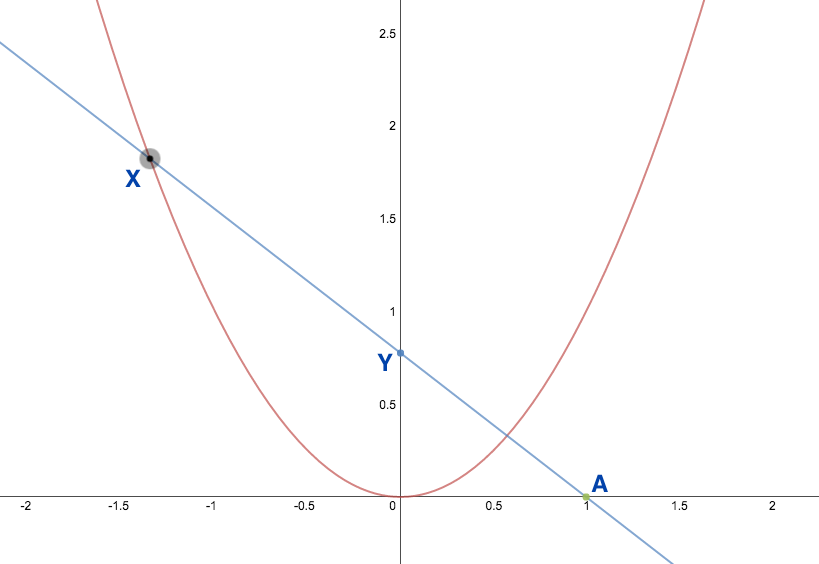
\includegraphics[width=0.7\textwidth]{01vectorproblem3.png}

(c) What is given, and what is unknown? Here $t$ is given. Varying $s$ will slide the point $Y$ with position vector $\vy$ along the line $\ell$. So we have to find an $s$ for which $Y$ is on the $y$-axis, and, since $t$ is given, our answer will depend on $t$. The point $Y$ is on the $y$-axis if its $x$-coordinate vanishes. So, we solve
\[ 
  1+s(t-1)=0 \implies s = \frac{1}{1-t}.
\] 
Hence the intersection point is $Y$ with the above value of $s$
\[ \vy = \vek 0\\ t^2/(1-t) \tor. \]
\endanswer

\problem
Consider the plane curve given by $\vx(t) = \vek t^2 \\ t^3 \tor$.

\subprob Find a parametric representation of the tangent line to the curve at the point with position vector $\vx(1)$.
  
\subprob Find a parametric representation of the tangent line to the curve at the point with position vector $\vx(a)$ for any value of the constant $a$.
\answer 
Chapter 2, section 3, tells you how to find the parametrization of a line.  Read that first before reading the rest of this answer.  To parametrize a line, you need one point on the line, and a vector in the direction of the line.

(a) The velocity vector is $\vx'(t) = \vek 2t \\ 3t^2 \tor$, so the velocity vector at $t=1$ is $\vx'(1) = \vek2\\3 \tor$. 
This vector is a tangent vector to the curve at the point $\vx(1) = \vek 1 \\1 \tor$. So the tangent
at this point is the line through $\vx(1)$ with direction $\vx'(1)$: 
\[ \vy(t) = \vek 1\\1\tor + t \vek 2\\3\tor\]
The $t$ in this parametrization is not the same as the $t$ in the parametrization $\vx(t)$ for the curve.
To avoid confusion, one sometimes chooses a different letter, for instance, 
\[ \vy(s) = \vek 1\\1\tor + s \vek 2\\3\tor \]
or, use a greek letter, 
\[ \vy(\alpha) = \vek 1\\1\tor + \alpha \vek 2\\3\tor. \]
 
(b) The velocity vector is still $\vx'(t) = \vek 2t \\ 3t^2 \tor$, so the velocity vector at $t=a$ is $\vx'(a) = \vek 2a\\3a^2 \tor$.
This vector is a tangent vector to the curve at the point $\vx(a) = \vek a^2 \\a^3 \tor$.
So the tangent at this point is the line through $\vx(a)$ with direction $\vx'(a)$:
\[ \vy(t) = \vek a^2\\a^3\tor + t \vek 2a\\3a^2\tor \]
\endanswer

\problem What sign does $\omega$ have in 
Figure~\ref{fig:circular-motion-the-force}~?  How would the figure change if we
change the sign of $\omega$?  Does the force $\vF$ on the object change if we
change the sign of $\omega$?

%% \problem While reading the definition of the curvature vector and especially after
%% seeing the not-so-nice formula \eqref{eq:curvature-vector-in-hideous-form} for the
%% curvature vector it is natural to think ``isn't there a simpler way to define
%% curvature?''  Here is one attempt.  The questions invite you to judge this
%% alternative definition of ``curvature'' on its merits.
%% 
%% For any parametric curve a tangent vector is given by $\vx'(t)$.  To see if the
%% curve deviates from being a straight line we simply check if $\vx'(t)$ changes,
%% and we can do this by computing the derivative of $\vx'(t)$.  So let us define
%% \[
%%   \vK(t) = \vx''(t),
%% \]
%% and let us see if this measures how much the curve is curved.  (As
%% mathematicians we can define whatever we want, and this definition is a lot
%% simpler than \eqref{eq:curvature-vector-in-hideous-form}.)
%% 
%% \subprob True or False:  \textit{if $\vK(t)=\vvv0$ for all $t$ then the curve is
%% a straight line} \dots ?
%% 
%% \subprob Compute $\vK(t)$ for $\vx(t) = \tvek t^2\\t^2\ttor$, and draw the curve
%% traced out by this particular vector function.
%% 
%% \subprob True or False: \textit{if $\vx(t)$ traces out a straight line then
%% $\vK=\vvv0$} \dots ?
%% 
%% \subprob Conclusion: To what extent does the statement ``$\vK=\vvv0$'' have
%% anything to do with the statement ``$\vx(t)$ traces out a straight line''?

\problem Suppose a point $P$ is rotating around a line $\ell$, keeping 
its distance to the line fixed at $r$, and moving in a plane perpendicular to
the line.  Suppose the point has angular velocity $\omega$: this means that
during a time interval of length $t$ the angle swept out by the line segment
connecting $P$ to $\ell$ is exactly $\omega t$.

In a previous math or physics class it was shown that the velocity of
the point $P$ is $\omega r$, where $r$ is the distance from $P$ to
the line $\ell$.

The \emph{angular velocity vector} is defined to be the vector
$\vvv\omega$ whose length is $\omega$, and that is parallel to the
line $\ell$.  There are two such vectors ($\pm \vvv\omega$).  By
definition $\vvv\omega$ points in the direction in which a screw
would move if it were turning in the same direction as the point $P$.

\subprob Assuming the line $\ell$ passes through the origin show from the 
drawing that the velocity vector of the point $P$ is $\vv$ is given by $\vvv\omega
\cp \vx$.  You can do this in two steps, namely:

%% \setlength{\itemindent}{0pt}
%% \setlength{\listparindent}{0pt}
%% \setlength{\labelwidth}{0pt}
\begin{list}{---}
  {\setlength{\leftmargin}{0pt}}
\item \itshape show that $\vvv\omega\cp\vx$ has the same direction as $\vv$,
\item \itshape show that $\vvv\omega\cp\vx$ has the same length as $\vv$.
\end{list}

\subprob Show that the acceleration vector is given by $\va =
\vvv\omega\cp(\vvv\omega\cp\vx)$.  (hint: don't use the drawing, but combine
the definitions of $\vv$ and $\va$, in 
\eqref{eq:velocity-of-vector-motion} and \eqref{eq:acceleration-vector-def}
and also the product rule; finally, keep in mind that you have just found that
$\vv=\vvv\omega\cp\vx$.)

\subprob If someone told you they had computed the acceleration vector
and found
\[
  \va =(\vvv\omega\cp\vvv\omega)\cp\vx,
\]
could they be right?
Explain!  What if they told you they got $\va =
\vvv\omega\cp\vvv\omega\cp\vx$?

\subprob True or False (explain your answers):

(a) $\vv\perp \vx$?\qquad (b) $\va\perp \vv$? \qquad (c) $\va$ and
$\vx$ are parallel?

\subprob Include the acceleration vector $\va$ in the above drawing.

\problem Consider the ``twisted cubic,'' 
i.e.~the curve given by $\vx(t) = t\ves1+t^2\ves2+t^3\ves3$.

\subprob Find a parametrization for the tangent to the curve at the point where
$t=1$.  Where does this point intersect the $xy$-plane?

\subprob For any given $t$ find the tangent line to the curve 
at the point $X(t)$, and find where this curve intersects the $xy$-plane.  

\answer

At any point the velocity vector is $\vx' (t)=\vek 1\\2t\\3t^2\tor$.
In particular when $t=1$ we get 
\[
  \vx(t)=\vek 1\\1\\1\tor, \qquad     \vx'(t)=\vek1\\ 2\\ 3\tor.
\]
Therefore the tangent at this point is given by 
\[
  \vx(t) \vek 1\\1\\1\tor + t \vek1\\ 2\\ 3\tor.
\]
This notation is however problematic, because it uses $\vx$ and $t$, which already have a meaning: $\vx$ is the vector function describing the curve, and $t$ tells us which point $X(t)$ we have in mind.  So we must choose different letters that have not been used yet, like $\vy$ and $s$.   A correct answer is then
\[
  \vy(s) = \vek 1\\1\\1\tor + s \vek1\\ 2\\ 3\tor.
\]
That solves part (a).

Part (b) has a similar solution, except now the value of $t$ is not restricted to be $t=1$. 
The parametric form of the tangent to the curve at the point $X(t)$ is given by
\[
  \vy(s) = \vek t\\t^2\\t^3\tor + s \vek 1\\ 2t\\ 3t^2\tor.
\]
The result depends on two parameters, $s$ and $t$.
The parameter $t$ selects a point $X(t)$ on the curve;  given $t$, the parameter $s$ selects a point on the tangent to the curve at the point $X(t)$.

Intersections with the $xy$-plane are found by setting the third coordinate of $\vy$ equal to zero.  You get $s=-t/3$, and thus 
\[
  \vy=\vek \tfrac23 t \\ \tfrac13 t^2 \\ 0 \tor
\]

\endanswer

\problem Compute the length of one full turn of the helix by taking the
parametrization given in \eqref{eq:helix-def} and computing the length of the
segment with $0\le \theta\le2\pi$.

After computing the length, consider this:  let $P$ be the perimeter of the
circle underneath the helix, and let $H$ be the height achieved by one full turn
of the helix.  Show that the length $L$ of the helix satisfies $L^2 = P^2+H^2$.


\problem There is a multistory parking ramp where the way out 
is a path in the shape of a helix that is wound around the outside of the
building.  As a car drives down this path at night its headlights shine a spot
on the ground.  Which curve is traced out by this light spot as the car drives
all the way down?

Make a good drawing.  Assume for simplicity that the center of the Parking ramp
is the $z$-axis.

\problem Compute the tangent, curvature, normal and binormal 
for the following curves

\subprob The parabola: $\vx(t) = \tvek t^2 \\ t\ttor$.  At which point  
on the curve is the curvature the largest?  

\subprob Neil's parabola: $\vx(t) = \tvek t^2\\ t^3\ttor$.  At which point on  
the curve is the curvature the largest?

\subprob The helix: $\vx(\theta) =\tvek R\cos \theta \\ R\sin \theta\\  
a\theta\ttor$ (see \S~\ref{sec:helix} for an explanation of the constants $R$ and
$a$).  At which point on the curve is the curvature the largest?

\subprob The graph of $y=e^x$  
by using the parametrization $\vx(t) = \tvek t \\e^{t}\ttor$.
Where on the graph is the curvature the largest?
\answer $\kappa(x) = \dfrac{e^x}
{\bigl(1+e^{2x}\bigr)^{3/2}}$.

To find the point with largest curvature: 
$\kappa'(t) = \dfrac{e^t} {\bigl(1+e^{2t}\bigr)^{5/2}}
\bigl(1-2e^{2t}\bigr)$, so the maximal curvature (smallest radius of
curvature) occurs when $x=-\frac{1} {2}\ln{2}$.
\endanswer

\problem A vector function $\vx(t)$ describes the motion of a point in space.  It is known that there is a constant vector $\vm$ such that the velocity $\vv(t)$ always satisfies $\vv(t) = \vm \times \vx(t)$.  Show that the quantity $\vm\cdot \vx(t)$ is constant.
\answer
To show that $\vm\dpp\vx(t)$ is constant we differentiate it with respect to time:
\[
\frac{d \vm\dpp\vx(t)} {dt} = \vm\dpp\vx'(t) = \vm\dpp\bigl(\vm\cp\vx(t)\bigr) = 0,
\]
because the cross product $\vm\cp\vx(t)$ is always perpendicular to the vector $\vm$.
\endanswer

\problem A vector function $\vx(t)$ describes the motion of a point in space.  It is known that there is a constant vector $\vm$ such that the velocity $\vv(t)$ and acceleration $\va(t)$ always satisfy $\va(t) = \vm \cp \vv(t)$.

Show that the quantity $\|\vv(t)\|^2$ is constant.

Then show that the angle between $\vm$ and $\vv(t)$ is constant (hint: look at the dot product $\vm\dpp\vv(t)$).

\problem A vector function $\vx(t)$ describes the motion of a point in space.  It is known that there is a constant number $K$ such that the acceleration $\va(t)$ always satisfies $\va(t) = -K \vx(t)$.  Show that the quantity 
\[
  f(t) = \|\vv(t)\|^2 + K \|\vx(t)\|^2
\]
is constant (where $\vv(t)$ is by definition the velocity vector) by computing $f'(t)$.
\answer
The product rule for dot-products implies that
\[
  \frac{d \|\vv(t)\|^2}{dt} 
  = \frac{d \vv(t)\dpp \vv(t)}{dt}
  =2\vv(t) \dpp \va(t)
\]
and also
\[
  \frac{d \|\vx(t)\|^2}{dt} 
  = \frac{d \vx(t)\dpp \vx(t)}{dt}
  =2\vv(t) \dpp \vx(t).
\]
Therefore 
\[
  f'(t) = 2\vv(t) \dpp \va(t) + K 2\vv(t) \dpp \vx(t).
\]
Factor out the common factor $2\vv(t)$ in both terms here to get
\[
  f'(t) = 2\vv(t) \dpp \bigl(\va(t) + K\vx(t)\bigr).
\]
Since we are given that $\va(t) = -K\vx(t)$, this last expression is zero.  Thus we have $f'(t) = 0$ for all $t$, which implies that $f(t)$ does not depend on time.
\endanswer

\problem Suppose a point $X(t)$ is moving through space, and suppose its position vector at time $t$ is $\vx(t)$.

Assume that the position vector $\vx(t)$ and the acceleration $\va(t) = \vx''(t)$  are parallel at every instant in time $t$.  

Explain why the vector $\vx(t) \times \vx'(t)$ does not depend on time by simplifying $\frac{d}{dt}\left(\vx(t)\times\vx'(t)\right)$.
\answer
  By the product rule for cross products of vector functions we have
  \[
    \frac{d \vx(t) \times \vx'(t)}{dt}
    =\frac{d\vx}{dt} \times \vx'(t) + \vx(t)\times \frac{d\vx'}{dt} 
    =\vx'(t) \times \vx'(t) + \vx(t) \times \vx''(t).
  \]
  The first term vanishes because the cross product of any vector with itself vanishes.  The second term also vanishes because $\vx(t)$ and $\vx''(t)$ are given to be parallel, and the cross product of two vectors that are parallel always vanishes.

  Therefore the derivative of $\vx\times \vx'$ vanishes at every moment in time.  This implies that $\vx\times\vx'$ does not depend on time, i.e.~it is constant.
\endanswer
%% \problem Show: a curve is plane if and only if its torsion vanishes 
%%($\tau = 0$).
%%
%%\problem Express $\vx'\cp\vx''$ in terms of $\kappa, \tau, \vT, \vN,
%%\vB$ and $\|\vx'\|$.
%%
%%\problem Let $A(h)$ be the area of the triangle with vertices 
%%$\vx(t-h)$, $\vx(t)$ and $\vx(t+h)$.  Compute $\DS \lim_{h\to 0}
%%\frac{A(h)}{h^3}$.  Hint: use a Taylor expansion $\vx(t+h) = \vx(t) +
%%h\vx'(t) + \frac{h^2}{2}\vx''(t) + o(h^2)$.

\problem Let two points $A(2, 2, 1)$ and $B(2,0,3)$ be given.
Find a parametric representation for the line through $A$ and $B$.
\answer
We need a point on the line (we choose $A$, although $B$ would be just as good).

We need a vector in the direction of the line.  Here we can choose either $\tpv AB$ or $\tpv BA$.  Let's choose the first.

We get
\[
\va = \tpv OA = \vek 2 \\ 2\\ 1 \tor,
\qquad
\tpv AB = \vek b_1 - a_1\\  b_2 - a_2\\ b_3 - a_3 \tor
= \vek 2-2 \\ 0-2\\ 3-1 \tor = \vek 0 \\ -2 \\ 2\tor
\]
A parametric equation for the line is
\[
\vx(t) = \va + t \tpv AB
= \vek 2 \\ 2\\ 1 \tor + t \vek 0 \\ -2 \\ 2\tor
= \vek 2 \\ 2-2t \\ 1+2t \tor .
\]
\endanswer


\problem The vector function $\vx(t) = \vek  \tan t \\ t \tor$ describes the motion of a point $X(t)$ in the plane.

\subprob Compute the velocity, speed, and acceleration of the point at any time $t$.
\answer
The velocity and acceleration are vectors.  They are the first and second derivatives of the position vector, so
\[
  \vv(t) = \vx'(t) = \vek 1/\cos^2 t \\ 1\tor, \qquad
  \va(t) = \vx''(t) = \vek 2 \sin t/\cos^3 t \\ 0\tor.
\]
The speed is the length of the velocity vector, i.e.
\[
  v(t) = \|\vv(t)\| = \sqrt{ \frac 1{\cos^4 t} + 1}.
\]
\endanswer

\subprob At which moment(s) in time $t$ are the point's velocity and acceleration perpendicular?
\answer
  Velocity and acceleration are perpendicular if their dot-product vanishes.  We compute the dot-product:
  \[
    \vv(t)\cdot\va(t)
    = \vek 1/\cos^2 t \\ 1\tor \cdot \vek 2 \sin t/\cos^3 t \\ 0\tor
    = 2\frac{\sin t}{\cos^5 t}.
  \]
  This dot-product equals zero if $\sin t=0$, i.e.~when $t=0, \pm\pi, \pm2\pi, \pm3\pi, \dots$.
\endanswer

\subprob Where does the tangent line to the curve at the point $X(t)$ intersect the $x$ axis?
\answer
  A parametrization of the tangent at the point $X(t)$ is given by 
  \[
    \vy = \vx(t) + s \vv(t).
  \]
  Here $t$ determines at which point on the curve we are finding the tangent, and $s$ is the parameter along the tangent line.  So we get
  \[
    \vy = \vek \tan t \\ t \tor + s \vek 1/\cos^2 t \\ 1 \tor
    = \vek  \tan t + s/\cos^2 t \\ t + s \tor.
  \]
  $\vy$ will be the position vector of a point on the $x$-axis if the second component of $\vy$ vanishes, i.e.~if $s=-t$.  Therefore the intersection point with the $x$-axis has position vector 
  \[
    \vy = \vek \tan t - t / \cos^2t \\ 0 \tor.
  \]

\endanswer

\subprob Find an integral for the length of the part of the curve for which $0\le t\le \pi/4$ (no need to compute the integral).
\answer
    The length of the segment is the integral of ``\textit{speed }d(\textit{time}),'' i.e.
\[
  \text{length} 
  = \int_0^{\pi/4} v(t)dt = \int_0^{\pi/4} \sqrt{\frac 1 {\cos^4 t} + 1} \, dt.
\]
Note: the original question asked for the length of the segment from $t=0$ to $t=\pi$.  This segment is infinitely long as it includes the $t$-value $t=\pi/2$, at which $\tan t \to\infty$.
\endanswer

\subprob How long is the part of the curve for which $0\le t < \pi/2$ (you can answer this question by drawing the curve instead of computing the integral).
\answer
This curve is infinitely long because $\tan t \to\infty$ as $t\to\pi/2$.
\endanswer



\noproblemfont
\end{multicols}

